\chapter{Selectivity, Efficiency, and Robustness of the LCA}

\section{Introduction}
Work from David Field's lab \parencite{golden2016conjectures,vilankar2017selectivity} proposes a single-neuron analysis technique that allows us to increase the complexity of our neuron models without significantly decreasing our understanding by characterizing the neuron’s response geometry in the form of iso-response contours.
They show that contours can be straight or bent, and if bent they can bend towards the origin (endo-origin) or away from it (exo-origin).
We build on this work and show that the LCA exhibits curved iso-response contours when trained on natural images as well as the MNIST dataset.
This curvature is a result of population nonlinear computations provided by the LCA's lateral inhibitory connectivity and indicates improved selectivity against perturbations that are orthogonal to the neuron's preferred stimulus.
First we directly measure the network's selectivity to full-field oriented grating stimulus and show improved performance over linear and pointwise-nonlinear networks.
Next we provide evidence supporting the hypothesis that improved selectivity results in a more efficient code of natural images.
Finally, we propose that this selectivity forces adversarial perturbation vectors to have angles that are more in line with data dimensions, producing more semantically meaningful perturbations.
We develop an analytic argument to support this claim for single-neuron adversarial attacks.
Furthermore, we demonstrate by experiment that our method successfully improves robustness to adversarial attacks for a classifier trained on our model's outputs.
We contribute a novel perspective for understanding adversarial attacks and population nonlinear networks. 

\section{Measuring iso-response contours}\label{sec:ch4_iso_contours}
Inferring causes from natural signals is a challenging problem faced by biological vision systems.
%For artificial vision, the neural network community has largely tackled this problem using feedforward discriminative models.
%An alternative approach is to use generative models, in which the network must attempt to explain data in terms of an internal model of the world.
In biological neural networks we see a preponderance of evidence that individual neurons are highly non-linear, recurrent, and laterally connected.
The LCA is a generative model with lateral connectivity and recurrent inference that exhibits a variety of linear \parencite{olshausen1996emergence} and non-linear \parencite{zhu2013visual} receptive field effects that are well matched to biological neurons.
Many of these effects can be explained using the model neurons' iso-response contours - an experimental method for determining stimulus combinations that result in equal activation from recorded neurons \parencite{golden2016conjectures}.
In the brain, the atomic unit of computation is generally considered to be the neuron, but most deep learning research has eschewed the individual neuron, possibly obfuscating the connections between biological and artificial neural networks.
We compare the iso-response contours of feed-forward, pointwise nonlinear discriminative and generative network architectures against a more biologically-consistent population nonlinear generative network architecture.
Pointwise nonlinearities are the more traditional form of nonlinearities and are seen in many deep neural network architectures and computational neuroscience models.
They are defined as nonlinearities that are a function of only a single neuron in a layer and include rectification, sigmoid, and hyperbolic tangent.
Population nonlinearities represent the alternative class, where the nonlinearity output is a function of multiple neurons in a set.
These include divisive normalization \parencite{carandini2012normalization, balle2016end} and the network nonlinearity present in sparse coding \parencite{rozell2008sparse, olshausen1997sparse}.

Consider that a $P$-pixel image can be thought of as a single point in $\mathbb{R}^{P}$.
To measure a target neuron's iso-response contours, we first choose a two-dimensional cross section (or plane) in the $P$-dimensional space that is defined by two orthogonal vectors.
For most of the work here, we will use the target neuron's feed-forward weights as one of the two vectors.
To determine the second axis of our image plane, we start by finding another neuron's weight vector that has a nonzero inner-product with our target neuron's weight vector (and thus they are not orthogonal).
Then, to get an orthonormal basis, we use the Gram-Schmidt process to find a vector orthogonal to our target neuron, but coplanar with our second neuron.
For competitive networks like the LCA, this method increases the likelihood of competition between neurons and thus increases the curvature. 
Each point in the 2-D plane can be injected back into the image space and will have a high degree of correspondence to relevant data features.
We use each point as input to the neuron model and then bin the points according to the neuron's output amplitude.
The bin boundaries reveal the iso-response contours of the target neuron.
The iso-response contours of linear neurons are straight: any input perturbation that is orthogonal to the weight vector will result in equal activation.
For pointwise nonlinearities, this remains true: because the nonlinearity is performed after a linear projection, the output must also produce straight iso-response contours.
By contrast, for a population nonlinearity the gradient of the activation function with respect to a small perturbation in the input is a function of all other neurons in the layer.
Consider: for a perturbation that is orthogonal to a target neuron's weight vector, it is generically the case that some other neuron will have a non-orthogonal weight vector, which can result in a net change in all neuron outputs.
Therefore, iso-response contours for population nonlinear neurons can be bent.
In figure \ref{fig:ch4_iso_contours} we demonstrate contours for linear and nonlinear neurons.

\begin{figure}[h]
    \centering
    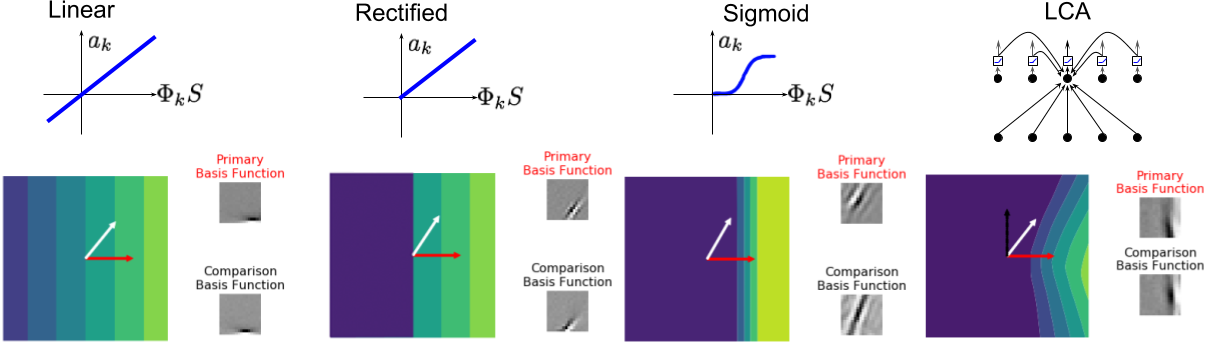
\includegraphics[width=\textwidth]{figures/iso_contour_comparison.png}
    \caption{\textbf{Empirically measured iso-response contours.} A fine sampling of points in a 2D plane are injected into the high dimensional image space and used as inputs to a target model neuron, $a_{k}$. The color value indicates a binned normalized response magnitude of the $k^{\text{th}}$ neuron, where purple indicates zero activity and yellow indicates the maximum. The red arrow is the weight vector for the neuron, $\Phi_{k}$. The white arrow is an alternate neuron's weight vector.}
    \label{fig:ch4_iso_contours}
\end{figure}

It is important to determine an individual neuron's response contours for a large number of planes to gain insight into its high-dimensional response geometry.
We propose two different methods for choosing image planes.
For both methods, we define one axis as the target neuron's weight vector.
The first method to find the orthogonal axis is to iteratively apply the process we described above for each other neuron in the layer.
For the second method, we compute a set of random vectors that are orthogonal to the target neuron’s weight vector.
We then estimate the curvature in each plane found via these two methods, which allows us to better understand the neuron’s high-dimensional iso-response geometry.
Figure \ref{fig:ch4_iso_contour_lca_hists} demonstrates that LCA neurons have negative curvature in nearly all planes tested.
Thus, most orthogonal perturbations from a neuron's weight vector will result in a decrease in its activation.
This is an important quality that we desire from our model neurons.
In visual neuroscience, we often use the neuron's linear receptive field (in our model that is represented by its weight vector) to represent the stimulus that the neuron is selective for.
With a pointwise nonlinear neuron model, it is possible to deviate away from its weight vector in many different directions without changing the neuron's response.
LCA neurons, on the other hand, have a higher degree of selectivity to perturbations away from their receptive field \parencite{vilankar2017selectivity}.
In the following section, we provide supporting evidence by comparing the orientation selectivity of the LCA against linear and pointwise nonlinear neuron models.
We also show that the LCA is more efficient than linear encoding models with oriented receptive fields, which we argue is a result of the improved selectivity.

\begin{figure}[h]
    \centering
    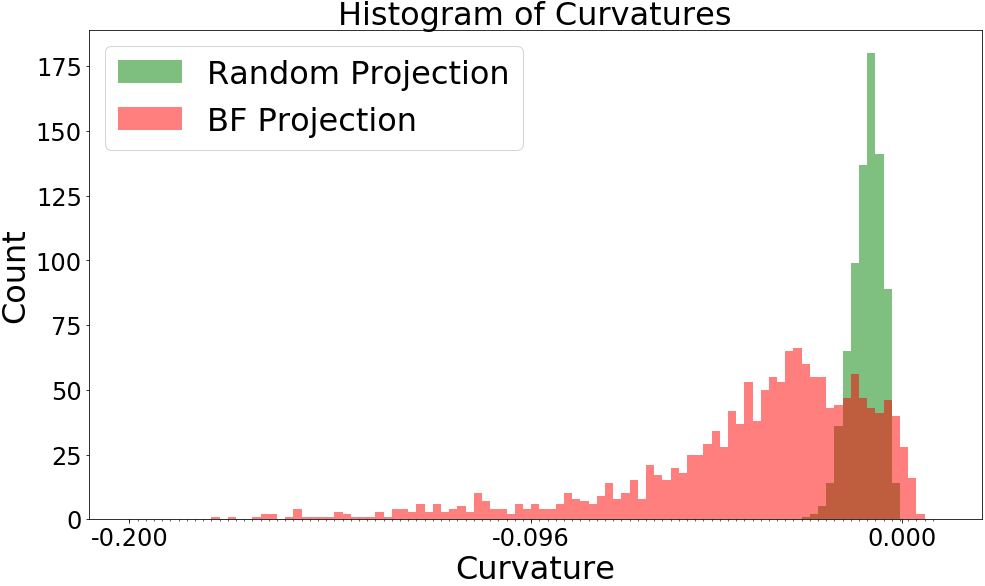
\includegraphics[width=0.8\textwidth]{figures/iso_contour_lca_hists.png}
    \caption{\textbf{LCA neurons have high-dimensional exo-origin curvature.} The histogram shows second order coefficients for polynomial fits to the lines in the middle plot. Negative coefficients indicate exo-origin curvature, which tells us that LCA neurons exhibit exo-origin curvature in almost all orthogonal directions tested. The target neuron was randomly selected from a 2x overcomplete LCA model trained on the MNIST dataset with z-score (zero mean, unit standard deviation) preprocessing. We replicated these results for many random neurons. See text for details about random versus targeted directions.}
    \label{fig:ch4_iso_contour_lca_hists}
\end{figure}


%TODO:
%\subsection{Hierarchical models exhibit endo-origin curvature}
% https://docs.google.com/presentation/d/1Vzk_fVGO-ERQDjKWRvzuHpV6YGwUriD6NyJNpf-WbVE/edit#slide=id.g4264a47c80_0_60
% would want to recompute curvatures for all neurons
% slide 80 covers lca+pca model, can show that curvature.
% then slide 73 gives subspace_lca curvature.


%TODO: include more schematic slides from oxyopia talk?
%https://docs.google.com/presentation/d/1Vzk_fVGO-ERQDjKWRvzuHpV6YGwUriD6NyJNpf-WbVE/edit#slide=id.g50750b3c61_0_158
%TODO: Include cross-orientation results?
%To assess the degree of orientation selectivity for ICA neurons, we replicate the cross-orientation suppression experiment performed by \parencite{zhu2013visual} with both sparse coding and ICA networks.
\section{Orientation selectivity and efficient coding}\label{sec:ch4_selectivity_efficiency}
A longstanding hypothesis in sensory neuroscience proposes that a primary function of early sensory processing is to form an efficient, redundancy-reduced code of the input that maximizes the brain's limited computational and biological resources while making explicit the statistical structure of the input \parencite{barlow2001redundancy}.
This hypothesis predicts that the response properties of sensory neurons should be adapted to the statistical structure of their input.
In support of this hypothesis, a number of the response properties of visual neurons have been reproduced by optimizing redundancy-reducing linear transformations on natural images.
For example, a symmetric decorrelation transformation of natural images yields center-surround receptive fields \parencite{atick1990towards}, and Principal Component Analysis (PCA) applied to color images yields the luminance, red-green, and blue-yellow channel observed in the opponent color coding of retinal ganglion cells \parencite{ruderman1998statistics, buchsbaum1983trichromacy}.
When higher-order correlations are additionally reduced, localized, oriented, and band-pass filters that resemble the orientation-selective receptive fields in V1 simple cells emerge \parencite{bell1997independent, olshausen1997sparse}.
It has thus been proposed that the oriented filters in V1 function to remove higher-order correlations.

Orientation selectivity is a striking feature of the response properties of simple cells in V1.
Since the discovery of orientation selectivity in Hubel and Wiesel's Nobel Prize-winning work, the mechanism for the computation has remained unclear.
A common point of confusion in the field has been the assumption that a neuron with a locally oriented receptive field will exhibit orientation selectivity.
Here, we will argue that narrow orientation selectivity requires a non-linear encoding process in addition to an oriented receptive field.
For experiments in this section all models were trained on natural image patches from the van Hateren dataset, which were transformed to log intensity, whitened, and normalized to have zero mean and unit variance \parencite{hateren1998independent}.

\subsection{LCA neurons have improved orientation selectivity}
Bent iso-response contours have important implications regarding the coding capabilities of neurons.
Work from David Field's lab \parencite{golden2016conjectures, vilankar2017selectivity} suggests that the degree of exo-origin curvature for neurons indicates how selective they are.
Here, we demonstrate this by showing that LCA neurons are more selective to oriented gratings than ICA neurons or neurons with pointwise sigmoid nonlinearities.
As we illustrate in figure \ref{fig:ch4_lca_selectivity_diagram}, linear or pointwise nonlinear neurons will respond equally to perturbations that are orthogonal to their weight vector.
However, if the target neuron has exo-origin bent contours, then any orthogonal perturbation from the neuron's weight vector will result in the activation decreasing.

\begin{figure}[h]
    \centering
    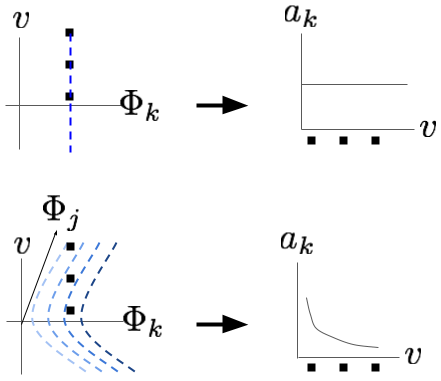
\includegraphics[width=0.4\textwidth]{figures/lca_selectivity_diagram.png}
    \caption{\textbf{Bent contours indicate increased selectivity.} This diagram shows qualitatively what expected responses would be for perturbations that are orthogonal to a neuron's weight vector. Each square represents an example input and the plots on the left indicate the inputs' positions in an image plane defined by the neuron's weight vector and an orthogonal vector. The plots on the right show what a model neuron's output would be for each type of nonlinearity. The bent contours indicate that a neuron's response will go down as one moves in an orthogonal direction from the weight vector in the image plane. This has important implications for neural coding - the neuron with bent contours is going to produce an activation value that is more indicative of the input's proximity to its weight vector.}
    \label{fig:ch4_lca_selectivity_diagram}
\end{figure}

We acknowledge that any degree of preference towards one orientation could be considered ``orientation selectivity''.
In the works of \parencite{golden2016conjectures,vilankar2017selectivity}, they alleviate this confusion by defining \textit{hyperselectivity} as a measure of the falloff in sensitivity as one moves away from a neuron's optimal stimulus, which is consistent with what we explained previously.
Instead of adhering to their mathematical definition of hyperselectivity, going forward we will refer to it qualitatively as narrow-band sensitivity to a type of stimulus.
Here we will only measure selectivity to changing orientation; we reserve measuring selectivity to other stimulus variations for future work.

% TODO: redo analysis with better SAE model
\begin{figure}[h!]
    \centering
    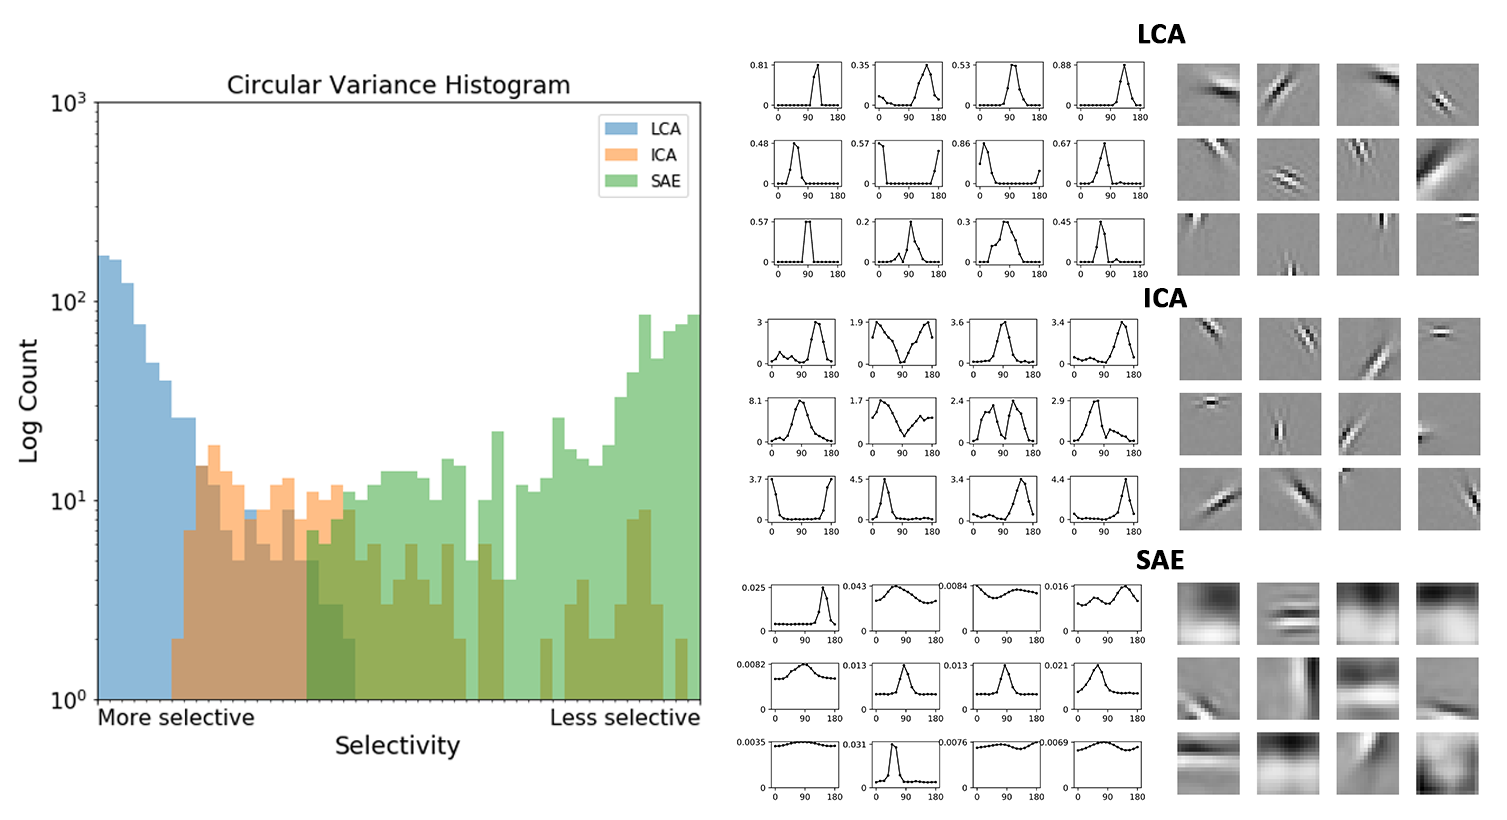
\includegraphics[width=\textwidth]{figures/circular_variance_histogram.png}
    \caption{\textbf{The LCA is more selective to oriented gratings than ICA or neurons with a sigmoid nonlinearity.} On the left is a histogram of the circular variance \parencite{ringach2002orientation}, a measure of orientation selectivity, for all of the neurons in each model. In the middle we show example orientation selectivity diagrams for neurons with different nonlinearities. On the right we show the corresponding weights for each of the orientation plots. The LCA and SAE networks had 768 latent units and the ICA network had 256. We also found that the shift in circular variance histograms as we increased overcompleteness (we tested 2x, 3x, and 4x overcompleteness levels) of the LCA was negligible compared to the difference between nonlinearities (data not shown).}
    \label{fig:ch4_orientation_selectivity}
\end{figure}


In figure \ref{fig:ch4_orientation_selectivity}, we compare the orientation selectivity of the LCA against ICA and a sparse autoencoder (SAE, \cite{ng2011sparse}).
We show that although all of the models can be trained to learn oriented filters, none of them are as selective to oriented grating stimuli as the LCA.
To produce the grating stimulus, we first computed the optimal spatial frequency for each neuron's weight vector using a Fourier transform.
Next, we constructed a set of full-field grating stimuli with the target spatial frequency, 16 different orientations, and 8 different phases.
Finally, we compute the neuron's circular variance to measure the orientation selectivity, which is a more generic measure than the traditional full-width at half-max in that it does not assume a Gaussian profile \parencite{ringach2002orientation}.

\subsection{Rate-distortion analyses}
Independent Component Analysis (ICA) is one of the most widely used image coding algorithms and has been proposed as a model for simple cells in V1 \parencite{bell1997independent, hyvarinen1999fast}.
The ICA algorithm explicitly optimizes for higher-order redundancy reduction, aiming to to reconstruct the input image as a linear superposition of a set of basis functions while minimizing the mutual information between the coefficients of data vectors in that basis.
Eichhorn et al. \citeyearpar{eichhorn2009natural} compare the coding efficiency of ICA and PCA to obtain the surprising result that ICA performs no better than PCA on a rate-distortion trade-off metric.
ICA is trained with the objective of minimizing the joint entropy of the activations and learns oriented filters that suggest it has succeeded in modeling higher-order pixel correlations, while PCA is a second-order method that does not learn oriented filters.
Eichhorn et al. \citeyearpar{eichhorn2009natural} argue that if ICA had succeeded at capturing higher-order statistics, it should show an advantage in the rate-distortion trade-off.
We present an alternate explanation of these findings by distinguishing \textit{orientation selectivity} from \textit{oriented filters}.
As we have discussed earlier in this chapter, neurons achieve narrow orientation selectivity via a nonlinear process.
We argue that although the ICA optimization algorithm is able to learn oriented filters, ICA's linear encoding process limits its capacity to perform orientation selectivity, which in turn limits its capacity to produce an efficient code.
Here, we replicate the rate-distortion analyses from \parencite{eichhorn2009natural} to show that the LCA's nonlinear encoding process produces lower entropy codes than linear encoders while being more perceptually robust to increasingly coarse quantization.

We trained LCA \parencite{rozell2008sparse}, ICA \parencite{bell1997independent}, and PCA (see \cite{jolliffe2016principal} for a recent review) on 1 million 16 x 16 pixel grayscale natural image patches.
Then, using the learned filter matrices, we computed model activations for a test set of 100,000 patches and uniformly quantized these activations with varying degrees of granularity.
For each level of granularity, we computed a reconstruction of the test input using the quantized activations and computed the mean squared error.
Figure \ref{fig:ch4_rate_distortion} plots the rate (mean marginal discrete entropy of the activations) against the distortion (mean squared error).
Results for the LCA trained with different values of $\lambda$ are also shown, where a larger $\lambda$ indicates higher sparsity.
We replicate the findings from \parencite{eichhorn2009natural} that (orthogonal) PCA  performs slightly better than ICA in the rate-distortion trade-off.
The LCA shows an advantage over both ICA and PCA.
Additionally, we find that representations that are more sparse are capable of achieving increasingly lower rates.

% TODO: Get sparsity (lambda) level for image plots - also, verify that it is off of the RD chart? - decided to take it out, could put it back in after the todo is solved
\begin{figure}[h]
    \centering
    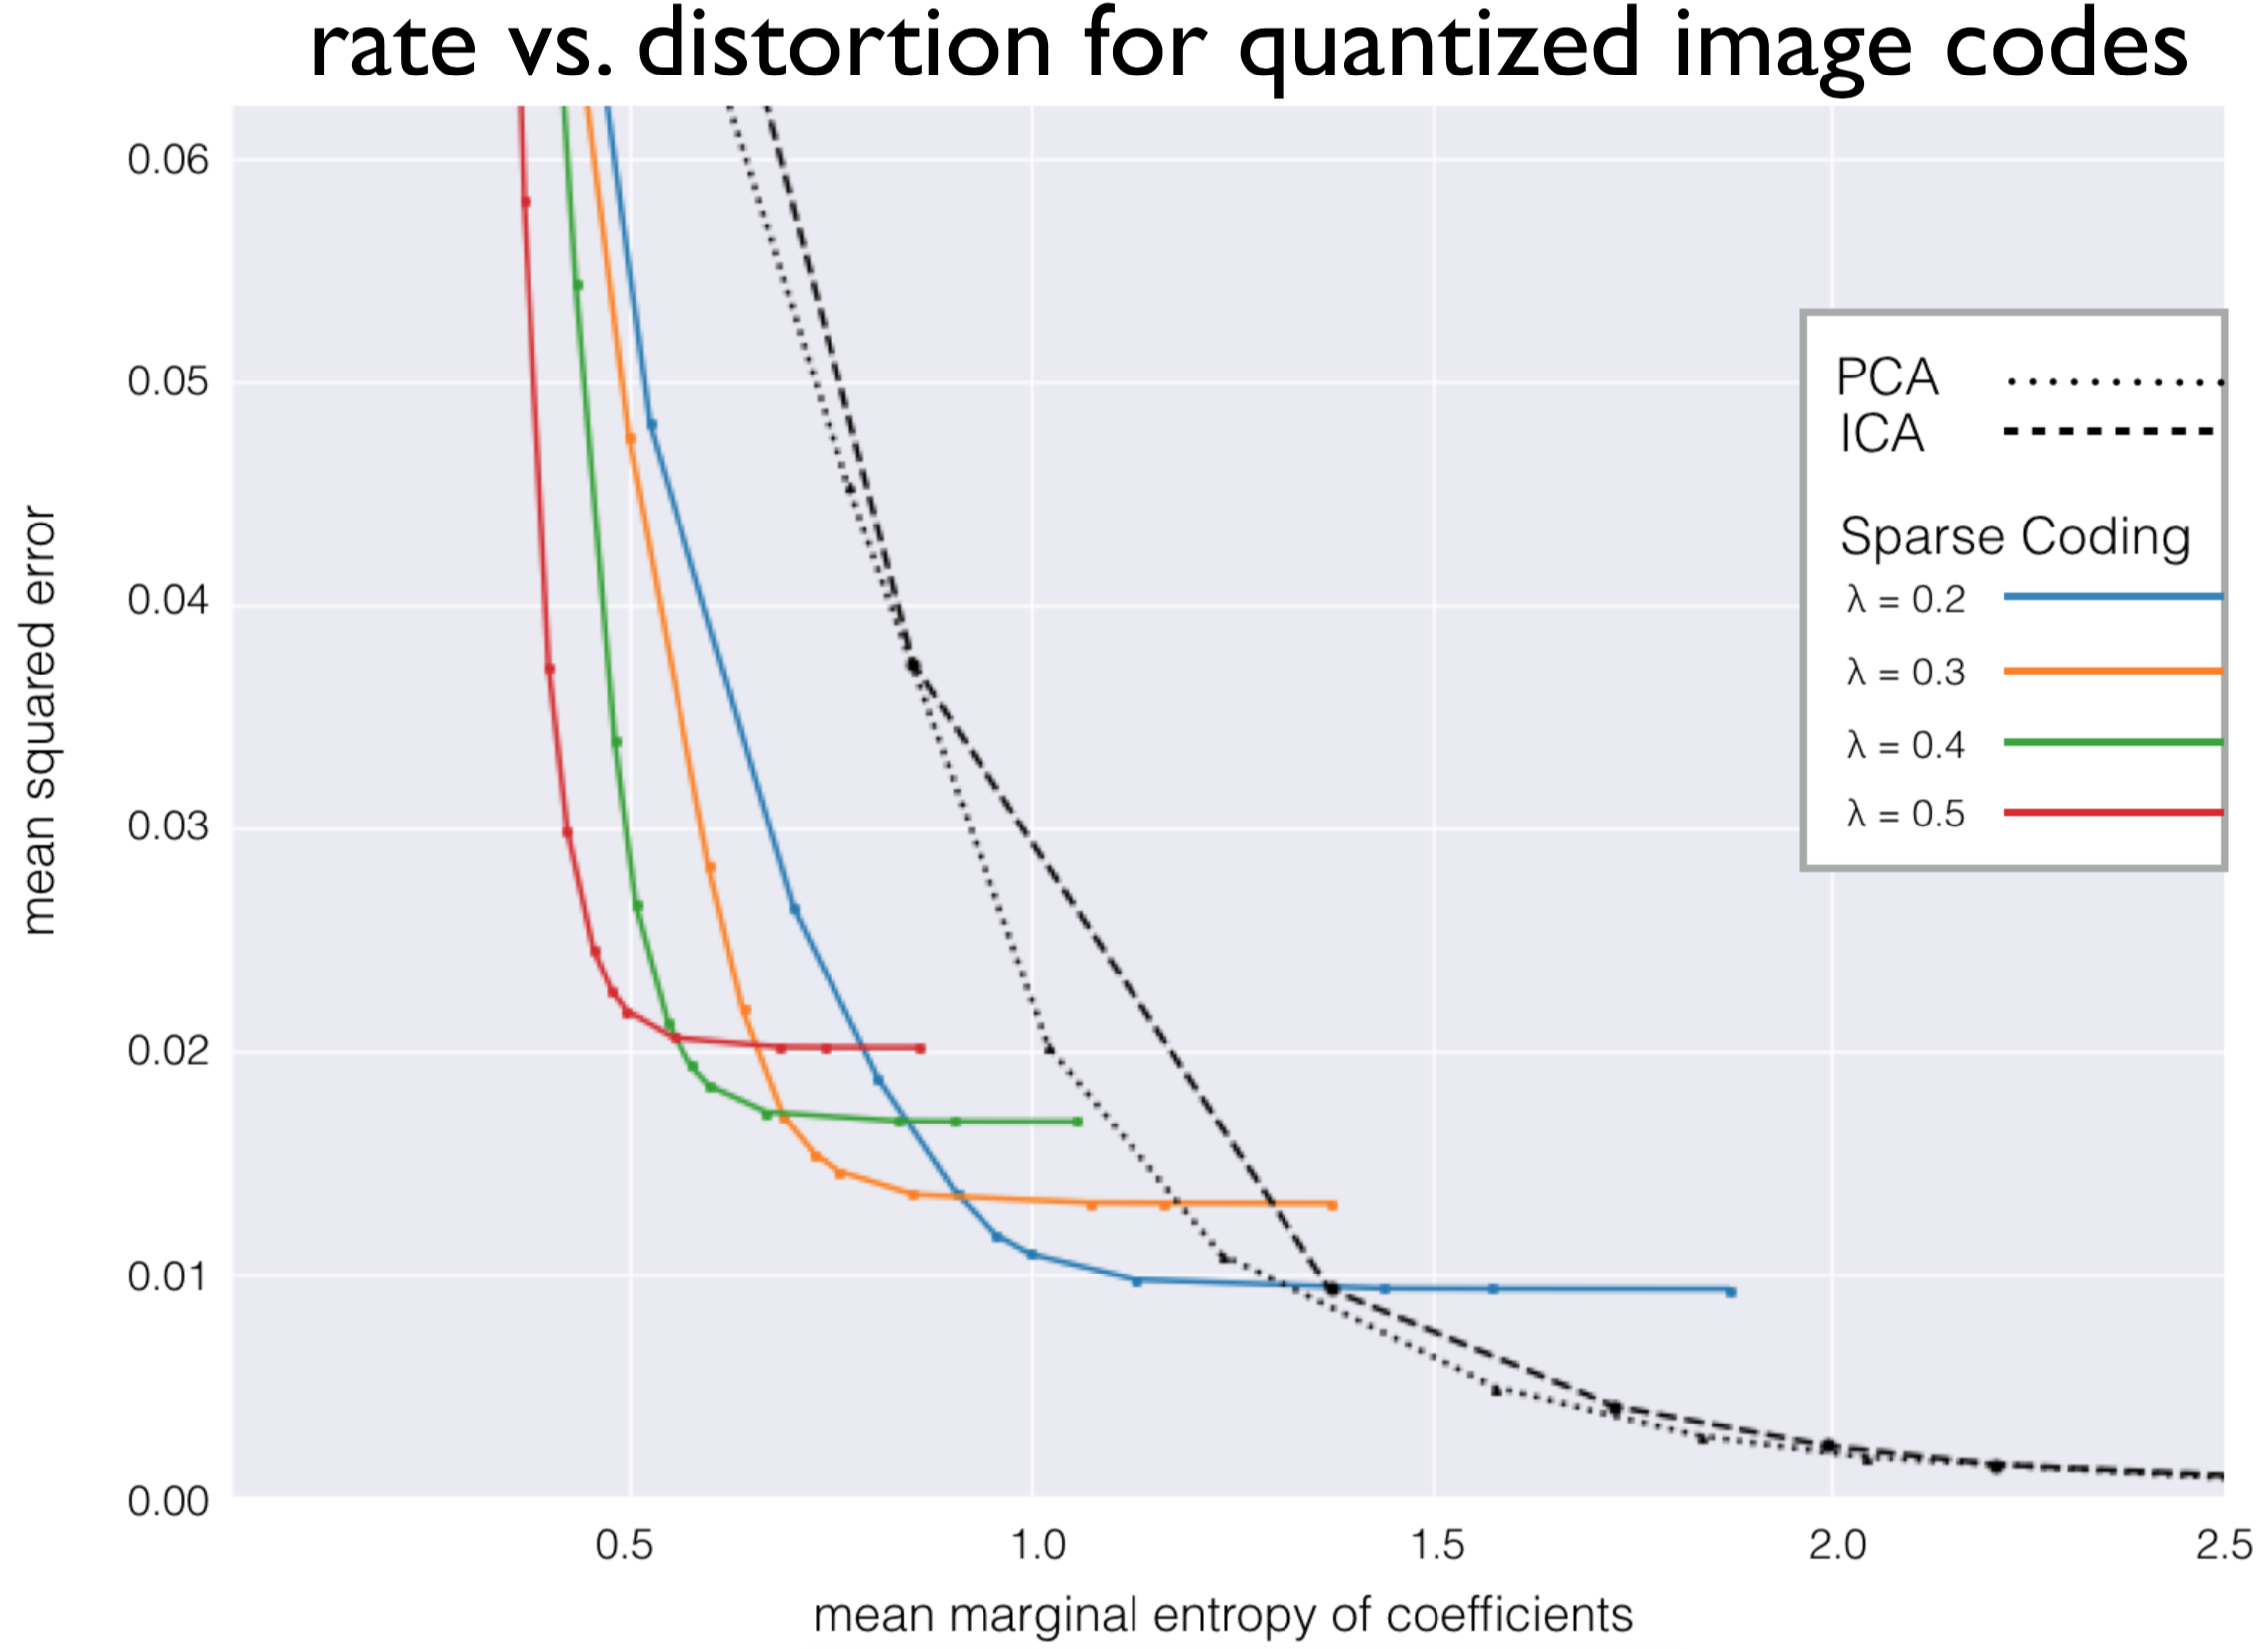
\includegraphics[width=0.7\textwidth]{figures/rate_distortion.png}
    \caption{\textbf{LCA provides better compression than ICA or PCA.} The rate-distortion plot compares the LCA trained with different sparsity levels against linear transforms. We replicate the finding from \parencite{eichhorn2009natural} that PCA performs slightly better than ICA in the rate-distortion trade-off, however the LCA shows an advantage over both PCA and ICA. Higher values of lambda indicates higher sparsity (i.e. fewer active elements). This figure was reproduced from unpublished work with permission from \parencite{sanborn2016sampling}.}
    \label{fig:ch4_rate_distortion}
\end{figure}


\subsection{Discussion}
Our results suggest the importance of nonlinear encoding for producing efficient codes of natural images and we demonstrate that narrowly orientation selective neurons are capable of reducing higher-order redundancy over second order linear transforms.
We demonstrate that the linear ICA neuron and the sigmoid nonlinear neuron used in the sparse autoencoder have broad orientation selectivity when compared to the LCA.
We also show that although the ICA algorithm is able to learn oriented filters, ICA's linear encoding process limits its capacity to perform genuine orientation selectivity, which in turn limits its capacity to produce an efficient code.

% TODO: Distribution shift experiment


\section{Iso-response contours predict adversarial attack directions}\label{sec:ch4_adv_defense}
Biological neurons are highly interconnected, both across and within layers, which gives rise to strong population nonlinear effects.
However, a large majority of research in neuron modeling uses pointwise nonlinearities due to the ease in interpretation and implementation.
Additionally, much of the research in adversarial analysis has focused on discriminative models \parencite{ng2002discriminative}.
Generative models, on the other hand, should not be as susceptible to adversarial attacks as discriminative models.
This is because they are trying to fit their internal model to the data as a ``sanity check'', which ideally should not succeed for adversarial perturbations.
Indeed, we identify classification of natural scenes as a perceptual problem, and we have argued in previous chapters that perception is a problem of inference.
In the absence of inference, the classification problem is insoluble, and adversarial examples are one aspect of that.
One method by which generative models can perform such a sanity check is via recurrent maximum a-posteriori (MAP) inference.
The LCA network uses population nonlinear interactions via lateral connectivity among neurons to facilitate this process, resulting in an ``explaining away'' effect commonly referenced in Bayesian inference literature \parencite{olshausen2013perception}.
This inference process also produces neurons that have exo-origin curved iso-response contours.
These two concepts are related, and the degree of exo-origin curvature can indicate how strong the explaining away effect is \parencite{vilankar2017selectivity}.
Here we bring these concepts together by comparing adversarial attacks against generative networks with curved iso-response contours and attacks against discriminative networks without.


\subsection{Adversarial Examples}
Adversarial examples are a demonstration of an artificial neural network's (ANN’s) inability to cope with distributional shift, which is any transformation that adjusts the distribution of inputs from that of the training data without changing semantic content \parencite{ford2019adversarial}.
They represent a worst-case demonstration of this weakness, which is a general problem that all classification ANNs are susceptible to \parencite{hendrycks2018benchmarking}.
We postulate that designing machine learning algorithms that are both accurate and robust to adversarial attacks requires a radical reformulation in how such algorithms are currently constructed.
In particular, we propose to allow our models to undergo a period of unsupervised learning that mimics the cognitive development of biological nervous systems instead of a strict reliance on reducing classification loss.
This is motivated by the observation that biological systems are robust to adversarial examples that affect deep networks.
However, in time-limited regimes that result in predominantly feed-forward brain computation, adversarial attacks have been shown to influence human decision making \parencite{elsayed2018adversarial}, suggesting that slower recurrent feedback loops aid in adversarial robustness.
Congruent with current theories for probabilistic inference in the brain \parencite{lee2003hierarchical}, we augment the standard ANN architecture with lateral connectivity and recurrence.
We propose that, together, these modifications will improve the network’s specificity to signals that lie along the data manifold.
We use adversarial attacks as a mechanism for understanding both traditional pointwise nonlinear ANNs and a population nonlinear alternative.

Adversarial attacks represent a flaw in typical deep neural networks where small targeted perturbations in the input space can cause large undesired changes in the output space.
Although the discovery of adversarial examples in deep networks is relatively new, it has had a considerable amount of academic attention and an understanding of these attacks has begun to emerge.
In the pioneering work of Szegedy et al. \citeyearpar{szegedy2013intriguing}, they introduce the idea of ``adversarial attacks'' for deep networks and propose that a non-smooth decision boundary in classification networks produces adversarial ``pockets'', or isolated regions on the data manifold, interspersed among dataset examples.
They also suggest that adversarial images represent a counter-example to the hypothesis that deep networks are able to achieve local generalization to input space regions in the vicinity of training examples.
Although this latter hypothesis has continued to hold, the presence of universal and transferable adversarial directions \parencite{moosavi2017universal} suggests that there are not adversarial pockets in the input manifold.
The follow up work of Goodfellow et al. \citeyearpar{goodfellow2014explaining} make several proposals, some of which have been refuted (for example by \cite{jetley2018friends}).
However, we would like to emphasize two important arguments from their work: 1) they present evidence suggesting that the direction of perturbation is more important than the specific point in space (further refuting the ``pockets'' theory), and 2) the adversarial perturbations are highly aligned with the weight vectors of a model.
The last of those observations has been explored in much more detail by Jetley et al. \citeyearpar{jetley2018friends}, who suggest that deep networks produce classification boundaries based on a small number of features that correspond to high curvature directions in the input space and that these high curvature directions are also the most effective adversarial directions.
The works of Gilmer et al. \citeyearpar{gilmer2018adversarial} and Ford et al. \citeyearpar{ford2019adversarial} further expand on this idea by suggesting that adversarial attacks confined to the $l_{\infty}$ box represent the worst-case example of the model's inability to account for distributional shift generally.

Recent work has also shown that nearly all proposed adversarial defense mechanisms fail in the face of more careful attacks \parencite{carlini2017towards, athalye2018obfuscated}.
For example, the recent defense method proposed by Sun et al. \citeyearpar{sun2018adversarial} claims to produce an adversarially robust preprocessing step, although they use basis pursuit in their methods, which possibly achieves robustness through gradient obfuscation \parencite{athalye2018obfuscated}.
However, their intuition that images should be forced onto the image manifold as a preprocessing step has great relevance to our work.
The work of Jacosen et al. \citeyearpar{jacobsen2018excessive} makes clear the trade-off between adversarial robustness and test accuracy and suggests that excessive invariance of a network should also be considered when understanding adversarial weakness.
Adversarial perturbations push inputs across decision boundaries such that the semantic quality of the image is largely the same but the label is changed to an incorrect classification.
It is also possible to arrive at the same result by generating an image such that the network's output is unchanged but the semantic quality is largely different, which they call an invariance-based adversary.
Our proposed framework is consistent with this idea and we provide an alternative perspective for excessive invariance.

The works of Kos et al. \citeyearpar{kos2018adversarial} and Goodfellow et al. \citeyearpar{goodfellow2014explaining} demonstrate the ability to produce adversarial examples for pointwise-nonlinear generative models that have applications in image denoising.
We would expect generative models to preserve information from their inputs and therefore be less susceptible to adversarial attacks.
Additionally, it has been suggested that denoising in general should help with robustness.
This work suggests a more nuanced explanation of adversarial susceptibility.

It will always be possible to produce an image perturbation that results in a change in class label, or an alternate reconstruction.
The academic interest in the subject comes from observations of how small that perturbation can be and the (lack of) semantic content of the perturbation.
Following the intuition provided in \parencite{ford2019adversarial}, successful defenses appear to require accounting for, or at a minimum detecting, distributional shift from the training data.


\subsection{Neuron response geometry predicts adversarial robustness}\label{sec:ch4_neuron}
In section \ref{sec:ch4_iso_contours}, we visualized the input-output maps of model neurons in the form of iso-response contours to better understand the difference between pointwise and population nonlinearities. Golden et al. \citeyearpar{golden2016conjectures} used iso-response contours to explain several non-linear properties as well as variance/invariance properties for V1 simple and complex cell models.
Vilankar and Field \citeyearpar{vilankar2017selectivity} further elaborate on this theory by proposing that neurons with exo-origin bent iso-response contours have a high degree of selectivity to their preferred stimulus.
In this section we propose to adopt this single-neuron iso-response analysis to better understand adversarial attacks on ANNs with varying degrees of biological realism.
We use iso-response contours as a lens to understand untargeted adversarial perturbations for individual neurons and predict important properties about the neurons' susceptibility to adversarial attacks.
We show that the response geometry of LCA neurons predicts data-aligned adversarial perturbations, resulting in semantically meaningful adversarial attacks.
We conduct our experiments on networks with both pointwise and population nonlinearities.
Although there are many types of networks that fit into these two categories, we focus this study on three specific instances: feedforward autoencoders (AEs), feedforward multi-layer perceptrons (MLPs), and the Locally Competitive Algorithm (LCA).
All analysis in this section was done using the MNIST dataset, which was normalized to have zero mean and unit variance.

Adversarial examples are closely tied to neuron iso-response contours.
While an iso-response contour represents a perturbation direction in stimulus space that produces no change in the output, an adversarial example is a perturbation direction that produces a maximal change in the output.
Below, we present analytic arguments that these two response directions are orthogonal for individual neurons.

If we extend the work of Marzi et al. \citeyearpar{marzi2018sparsity} to include nonlinear functions, then we can define adversaries as seeking to maximize the following objective, $\Delta$, with respect to a perturbation, $e$:

\begin{align}\label{eq:ch4_adv_metric}
\begin{split}
    \max_{e} \Delta (s, s+e) = \max_{e} |f(s+e) - f(s)| \\
    s.t. \|e\|_{\infty} < \varepsilon,
\end{split}
\end{align}

where $f(\cdot)$ can include a non-linear activation function, $s$ and $e$ are equal sized column vectors representing the data and perturbation, respectively, and $\varepsilon$ is some small scalar value.
To solve this equation, one must find a perturbation that results in a model output that is maximally different from the output with respect to the original input.
For our analysis, $e$ indicates a targeted perturbation of fixed magnitude that is subject to $\|e\|_{\infty}<\varepsilon$.
By definition, for any vectors $u$ and $v$, $\langle u,v\rangle = |u| \cdot |v| \cdot \mathrm{cos}(\Theta_{u,v})$.
Going forward, we will reference the inner angle between two vectors as $\Theta_{u,v}$ for some vectors $u$ , $v$.
If we assume that the perturbation magnitudes are fixed and equal, i.e.$\|e_{adv}\| = \|e_{iso}\| = k < \varepsilon$, then we can optimize over the angle between the perturbation vector and the input signal $\Theta_{e,s}$.
We can now include perturbation directions that result in a minimal change in the neuron's output:

\begin{center}
    \begin{tabular}{ |c | c| } \hline
     \textbf{Adversarial} & \textbf{Iso-Response} \\ \hline
     $\max_{\Theta_{e,s}}|f(s+e) - f(s)|$ & $\min_{\Theta_{e,s}} | f(s+e) - f(s) |$ \\ \hline
    \end{tabular}
\end{center}

These iso-response directions define contours in the neuron's response field.
We can use the Fr\'{e}chet definition of the derivative to better understand how the neural response geometry relates to adversarial images:

\begin{align}\label{eq:ch4_frechet}
\begin{split}
    f(s+\varepsilon) &= f(s) + \langle\nabla_{s}f(s), \varepsilon\rangle + o(\varepsilon)\\
    &\therefore \\
    f(s+\varepsilon) - f(s) &= \langle\nabla_{s}f(s), \varepsilon\rangle+ o(\varepsilon),
\end{split}
\end{align}

where $\langle , \rangle$ indicates a dot product and $o(\varepsilon)$ is a tight bound that means ``terms that are, in the limit $\varepsilon \rightarrow 0$, dominated by $\varepsilon$''.
This is of similar character to a Taylor series expansion. We can now combine these ideas to rewrite the adversarial and iso-response attack objectives:

\begin{align}\label{eq:ch4_angle_metric}
\begin{split}
    &\textbf{Adversarial:} \max_{\Theta_{e,s}} |\nabla_{s}f(s)^\top e + o(\|e\|)|,\\
    &\textbf{Iso-Response:} \min_{\Theta_{e,s}} |\nabla_{s}f(s)^\top e + o(\|e\|)|,
\end{split}
\end{align}

where $\nabla_{s}f(s)$ is the output gradient of the target neuron.
For small $\|e\|$, the linear terms in equation \eqref{eq:ch4_angle_metric} dominate and these equations are solved when $e \parallel \nabla_{s}f(s)$ for the adversarial perturbation and $e \perp \nabla_{s}f(s)$ for the iso-response perturbation.
This tells us that the optimal adversarial directions will always be perpendicular to the iso-response directions for an untargeted adversarial attack. 

\subsubsection{Estimating adversarial directions}
The response function of a model neuron for a perturbation, $e$, added to an input signal, $s$, can give us insight to that neuron's iso- and adversarial-response properties. First, we will describe this for a linear neuron, $f_{k}(s) \coloneqq \phi_{k}^\top s$:

\begin{align}\label{eq:ch4_linear_neuron}
\begin{split}
    f_{k}(s+e) &= \phi_{k}^\top (s + e) \\
    &= \phi_{k}^\top s +\phi_{k}^\top e,
\end{split}
\end{align}

where $\phi_{k}$ is a column weight vector. Next we match equation \eqref{eq:ch4_linear_neuron} to the top part of equation \eqref{eq:ch4_frechet}:

\begin{equation}
    f(s) + \langle\nabla_{s}f(s), e\rangle + o(\|e\|) = \phi_{k}^\top s + \phi_{k}^\top e.
\end{equation}

This tells us that the first term on the right hand side is $f(s)$ and the second term is $\langle\nabla_{s}f(s), e\rangle$, which means the third term is $o(||e||)=0$ (this is expected because it is a linear function). Therefore,  $\nabla_{s}f(s) = \phi_{k}$ and for any $e \perp \phi_{k}$, $f_{k}(s+e) = f_{k}(s)$.

For a fixed amplitude perturbation, the maximum adversarial direction is when the inner angle $\Theta_{\phi_{k},e} = 0$. Additionally, perturbations that are orthogonal to $\phi_{k}$ are iso-response directions because they do not change the function's output, which is illustrated in figures \ref{fig:ch4_iso_contours} and \ref{fig:ch4_lca_selectivity_diagram}.

We can again use equation \eqref{eq:ch4_frechet} to gain insight about the iso-response directions and adversarial directions for pointwise nonlinear functions, such that $f_{k}(s) \coloneqq g_{k}(\phi_{k}^\top s)$:

\begin{align}\label{eq:ch4_pw_nonlin}
\begin{split}
  f_{k}(s+e) &= g_{k}(\phi_{k}^\top(s+e)) \\
  &=g_{k}(\phi_{k}^\top s + \phi_{k}^\top e) \\
\end{split}
\end{align}

where $g_{k}(\cdot)$ is a pointwise non-linear activation function for neuron $k$. If we perform a change of variables such that $a = \phi_{k}^\top s$ and $b = \phi_{k}^\top e$, then we can fit equation \eqref{eq:ch4_pw_nonlin} to match equation \eqref{eq:ch4_frechet}:

\begin{align}\label{eq:ch4_pw_nonlin_frechet}
\begin{split}
    f_{k}(s + e) = g_{k}(a + b) &= g_{k}(a) + \nabla_{s}g_{k}(a) \cdot b + o(b) \\
    &=g_{k}(\phi_{k}^\top s) + \nabla_{s}g_{k}(\phi_{k}^\top s) \cdot \phi_{k}^\top e + o(\phi_{k}^\top e)\\
    &=g_{k}(\phi_{k}^\top s) + \langle\nabla_{s}g_{k}(\phi_{k}^\top s) \cdot \phi_{k}^\top, e\rangle + o(\|e\|),
\end{split}
\end{align}

Now we match equation \eqref{eq:ch4_pw_nonlin_frechet} to the bottom part of equation \eqref{eq:ch4_frechet} to show 

\begin{equation}
\begin{split}
    |f_{k}(s+e) - f_{k}(s)| = |\nabla_{s}g_{k}(\phi_{k}^\top s) \cdot \phi_{k}^\top e + o(\|e\|)|.
\end{split}
\end{equation}

Again, the function is maximized when $\phi_{k} \parallel e$ and minimized when $\phi_{k} \perp e$, which tells us that a pointwise nonlinearity can only change the spacing between the contours, it cannot bend the contours in any way.

Finally, we extend this analysis to population nonlinear networks.
For population nonlinear networks, the output is now a function of the the other neurons in the layer as well as the input.
Thus, $\Phi$ represents the entire weight matrix, with rows set to $\phi_{k}^\top$.
To determine the activation of a single neuron, $k$, we use a one-hot selection vector, $p_{k}$.
Thus, we define the activation function, $f_{k}$ as:

\begin{align}\label{eq:pop_nonlinear}
\begin{split}
   f_{k}(s+e) &\coloneqq p_{k}^\top g(\Phi(s+e)) \\
   &= p_{k}^\top g(\Phi s + \Phi e) \\
   &= p_{k}^\top g(\Phi s) + (\nabla_{s}g(\Phi s)^\top p_{k})^\top \Phi e + o(\|\Phi e\|) \\
   &= p_{k}^\top g(\Phi s) + (\Phi^\top \nabla_{s}g(\Phi s)^\top p_{k})^\top e + o(\|e\|),
\end{split}
\end{align}

where $g(\cdot)$ is a function of the weight matrix times the input, and $\nabla_{s}g(\Phi s)$ is its Jacobian.
We can no longer simply describe the contours of these neurons because the gradient of the non-linearity is now a function of (an arbitrary linear transformation of) $s$.
Thus, for individual neurons, the contours can be straight or bent.

Although we know that the adversarial directions are perpendicular to iso-response contours, we cannot analytically derive the directions for population nonlinearities.
Instead, we can estimate adversarial perturbation directions by measuring the iso-response contours empirically.
Figure \ref{fig:ch4_adv_grads} shows schematic drawings of the contours measured for population- and pointwise-nonlinear neurons along with the expected adversarial directions.

\begin{figure}
    \centering
    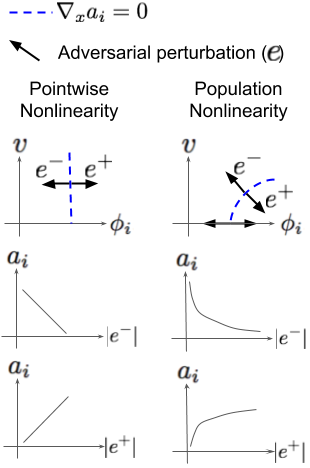
\includegraphics[width=0.3\columnwidth]{figures/adversarial_gradients_iso_contours.png}
    \caption{\textbf{Schematic description of adversarial attacks relative to iso-response contours.} Adversarial gradients (dark arrows) are always orthogonal to the iso-response contours (blue dashed line).$\Phi_{k}$ indicates a weight vector for the neuron $a_{k}$, and $v$ represents a random orthogonal direction.}
    \label{fig:ch4_adv_grads}
\end{figure}

\section{The LCA provides defense against adversarial attacks}
Recall that the adversarial objective in equation \eqref{eq:ch4_adv_metric} has an absolute value and is thus bi-directional.
For a locally linear approximation of an untargeted attack, these two directions are equal.
However, if we impose a rectifying constraint on our neuron outputs, then the two solutions are not equal for an individual neuron.
For a sufficiently large $e$, the direction that lowers the neuron's output to below threshold will result in $f(s+e)=0$, i.e. $\max_{e^{-}}|f(s+e)-f(s)| = f(s)$.
This means that, for rectified units, $\max_{e^{-}}|f(s+e)-f(s)|$ could be less than $\max_{e^{+}}|f(s+e)-f(s)|$.
This would not be known to a simple gradient method for computing a non-targeted adversarial attack, such as that proposed in equation \eqref{eq:ch4_adv_metric}.
However, in practice actual adversarial attacks have an additional goal in mind: to produce an output corresponding to some other data sample.
Turning off all of the units in a layer is not a solution to this problem, so some set of adversarial perturbations must be in the $e^{+}$ direction.
By definition, these perturbations will have greater contribution to the model's output than $e^{-}$ perturbations.

If the LCA is rectified, then the $e^{-}$ direction will eventually turn off units.
From figure \ref{fig:ch4_adv_grads} one can deduce that the only $e^{+}$ direction that will cause the output of neuron $k$ to grow without bound is along $\Phi_{k}$.
What's more, \emph{all} directions that increase that neuron's output are towards, or along, $\Phi_{k}$.
From this analysis we hypothesize that adversarial attacks on networks with exo-origin bent contours will be more aligned with the their weight vectors than attacks on networks with straight contours.
If the weight vectors are data aligned then this will result in adversarial attacks that are data aligned.
Recall from section \ref{sec:ch4_iso_contours} that the LCA has exo-origin curvature in nearly all orthogonal directions.
Therefore, the high-dimensional iso-response geometry is that of an irregular hyper-cone, which indicates protection from orthogonal perturbations.
In figure \ref{fig:ch4_marzi_network_attack}, we show that the LCA network has qualitatively more data-aligned perturbations for an untargeted attack when compared to rectified and sigmoid autoencoders with a single hidden layer.
The rectified network performed worse, likely because of the unbounded nature of the activation function.
However, even the bounded sigmoid network produced noisy adversarial images with pixels that are irrelevant to the stimulus space becoming active.

\begin{figure}[h]
    \centering
    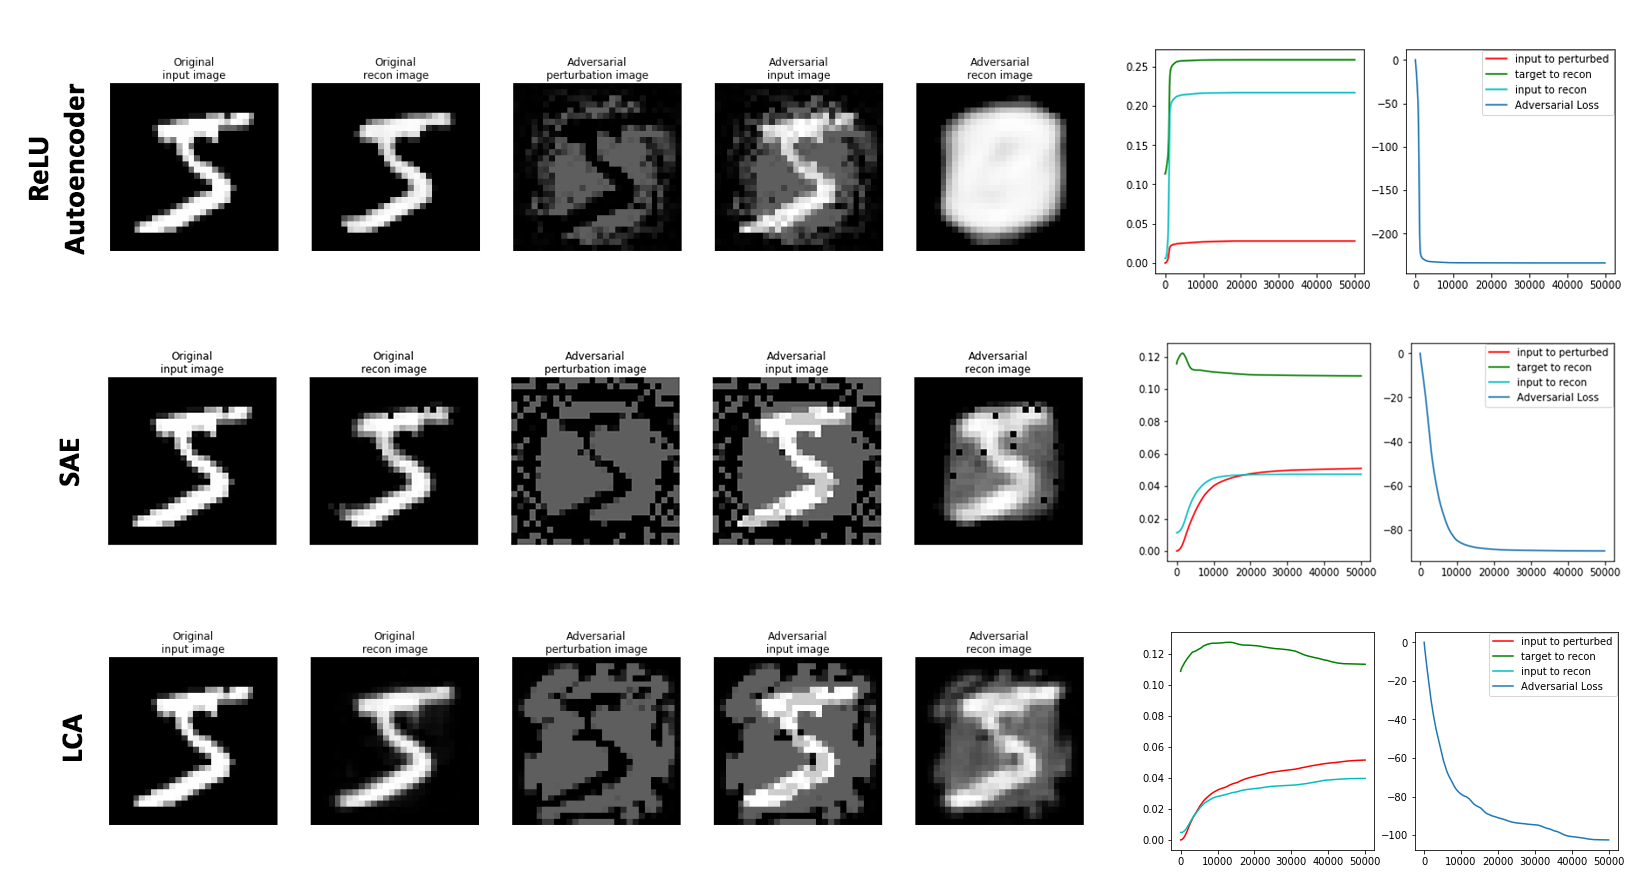
\includegraphics[width=\textwidth]{figures/adv_network_marzi_lca_sae_relu.png}
    \caption{\textbf{LCA results in more data-aligned adversarial attacks.} Here we compare the LCA against shallow (single hidden layer) autoencoders with rectified and sigmoid nonlinearities. Although all three networks learn similar structured basis functions, the LCA model shows the most data-aligned adversarial perturbations. The attack for this figure follows equation \eqref{eq:ch4_adv_metric}, which is an untargeted attack on the network output. All networks in this experiment had 768 hidden units.}
    \label{fig:ch4_marzi_network_attack}
\end{figure}



\subsection{Untargeted attacks}\label{sec:ch4_deep_relu_comparisons}
Deep networks can approximate complex functions if they have enough training data. Therefore, it is reasonable to expect a deep network to learn to produce exo-origin bent iso-response contours from neurons in its latent space if efficiency or selectivity is a primary goal of the model. To test this, we trained a deep rectified bottleneck autoencoder and measured its iso-response curvature as well as its susceptibility to single-unit untargeted adversarial attacks. The autoencoder is trained to produce high quality reconstructions (approximately matched to the LCA) while communicating the information through a restricted channel of 64 neurons, which should encourage an efficient representation. We were unable to train a deep architecture with a sigmoid activation that learned structured weights for comparison. Figure \ref{fig:ch4_drae_curvature} shows that the autoencoder learns both exo- and endo-origin curvatures, which makes the quality of adversarial attacks less easy to predict. To produce the curvature plots, we had to select a relevant image plane for the target neuron. Following the methods outlined in \parencite{mahendran2016visualizing}, we used gradient ascent to find an optimal stimulus for a given latent neuron. We then followed the same procedure as outlined for figure \ref{fig:ch4_iso_contours} with the neurons' optimal stimuli as our target and comparison vectors.

% TODO: Get histogram plot
\begin{figure}
    \centering
    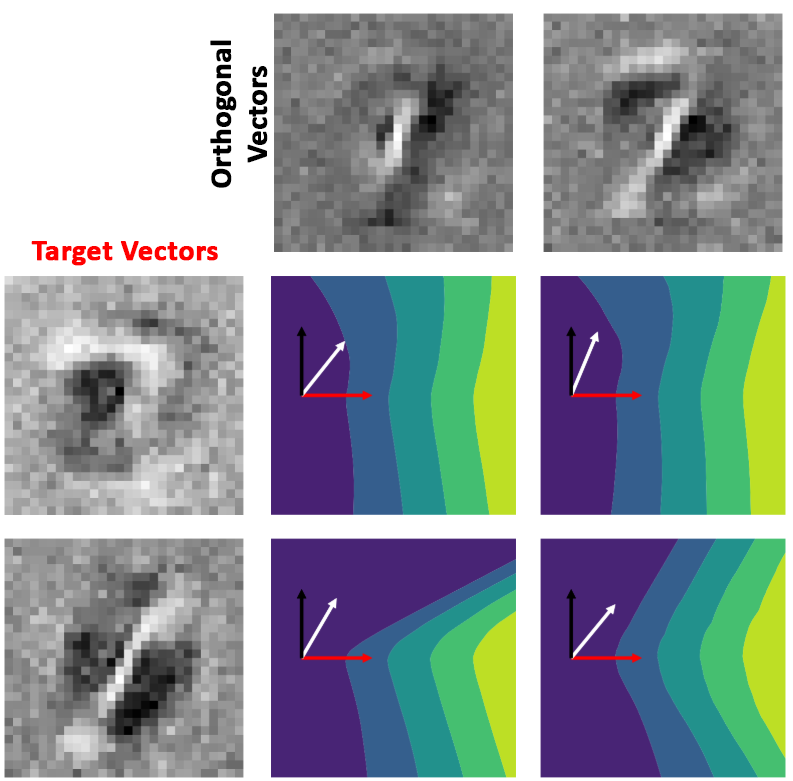
\includegraphics[width=0.5\textwidth]{figures/drae_deep_curvature.png}
    \caption{\textbf{Deep ReLU autoencoders exhibit non-uniform curvature.} The left plot shows example curvatures for the autoencoder neuron. On the right, a single neuron was selected and curvatures were computed following the procedure used for figure \ref{fig:ch4_iso_contour_lca_hists}.}
    \label{fig:ch4_drae_curvature}
\end{figure}

In figure \ref{fig:ch4_marzi_unit_relu_lca}, we show that if we perform the attack defined in equation \eqref{eq:ch4_adv_metric} on a single neuron, such that we minimally change the input while maximally activating a single neuron, then the output for the deep ReLU autoencoder becomes similar to that neuron's optimal stimulus. However, the LCA network simply enhances the feature associated with the target neuron without destroying other structure in the image.

\begin{figure}[h]
    \centering
    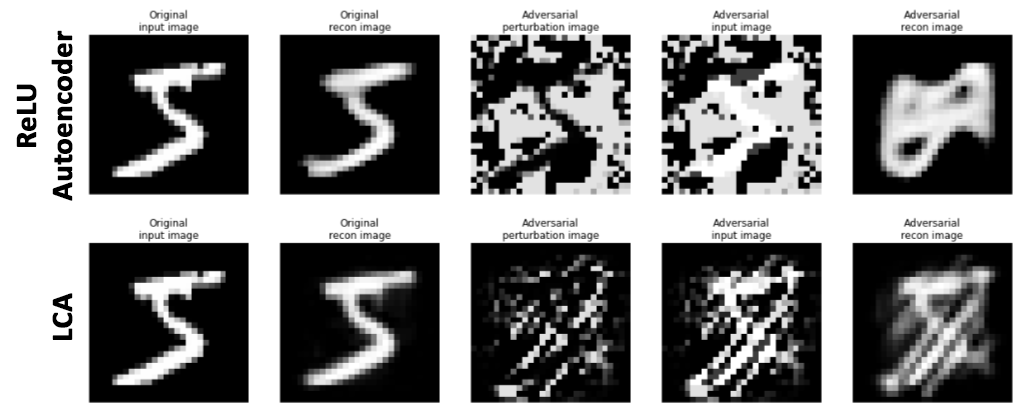
\includegraphics[width=\textwidth]{figures/adv_marzi_unit_relu_lca.png}
    \caption{\textbf{LCA preserves image structure with single unit adversarial attacks.} We attack individual latent units in a deep rectified autoencoder and the LCA. The attack destroys any structure corresponding to the original digit class for the rectified autoencoder, but the structure is largely preserved for the LCA attack.}
    \label{fig:ch4_marzi_unit_relu_lca}
\end{figure}


\subsection{Targeted attacks}\label{sec:ch4_mnist_experiments}
For the targeted MNIST experiments, we followed the procedures outlined in \parencite{kos2018adversarial, kurakin2016adversarial, carlini2017towards} to construct various adversarial attacks. We consider the LCA as an autoencoder model, $\hat{s}=g(f(s))$, which encodes images into a latent space, $a=f(s)$, and then produces reconstructions from this encoding, $\hat{s}=g(a)$. We compare the LCA against the following models:

% TODO: Check parameters / weight decay / etc for MLP
% TODO: This list should probably go earlier in the section
\begin{itemize}
  \item A sparse autoencoder (SAE, \cite{ng2011sparse}) with a single overcomplete (768 units) hidden layer that uses a pointwise sigmoid nonlinearity.
  %\item A pointwise rectified (ReLU) \parencite{hahnloser2000digital, nair2010rectified} autoencoder with a single overcomplete (768 units) hidden layer.
  \item A deep bottleneck pointwise rectified (ReLU) \parencite{hahnloser2000digital, nair2010rectified} autoencoder with 5 encoding layers that have 768, 256, 256, 128, and 64 units, a dropout keep probability of 50\%, 70\%, 70\%, 70\%, and 100\%, and a mirrored decoder.
  \item A deep variational autoencoder \parencite{kingma2013auto} with three encoding layers that have 768, 512, and 50 units, respectively, with a mirrored decoder. We used the leaky-ReLU activation function \parencite{maas2013rectifier} with dropout keep probability of 80\% for the first and last two layers and 100\% otherwise. We also used a weight decay regularization loss with a trade-off multiplier of 0.003. 
  \item A two-layer ReLU multi-layer perceptron (MLP) discriminative model.
  \item An alternative implementation of the ISTA sparse coding framework called Learned ISTA, \parencite{gregor2010learning}.
\end{itemize}

In figure \ref{fig:ch4_adversarial_mlp_vs_lca}, we show that the LCA requires stronger adversarial perturbation magnitudes to achieve the same change in the network output when used as an initial encoding layer for classification tasks. In figure \ref{fig:ch4_kos_generative_attack}, we show the improved robustness of the LCA against more standard feedforward autoencoders using a generative adversarial attack. Adversarial perturbations for the LCA are more aligned with the data than those for the alternative models tested, which we demonstrate in figures \ref{fig:ch4_adversarial_mlp_vs_lca} and \ref{fig:ch4_cosine_similarity}. We also found that for attacks that did not include a clipping step to force the perturbation to be a certain size, the SAE perturbation grew without bound while the LCA perturbation settled to a fixed distance from the input (figure \ref{fig:ch4_lca_sae_unbounded_attack}). We have shown that these properties can be explained by an LCA neuron's exo-origin bent iso-response contours. We believe that this study synergizes with the works of \parencite{zhu2013visual, golden2016conjectures, vilankar2017selectivity, olshausen1997sparse}, which together suggest that the explaining-away process inherent in the sparse coding model produces a more selective and robust code of input data.


\subsubsection{Comparisons against a sparse autoencoder}
In section \ref{sec:ch4_adv_defense}, we proposed that adversarial gradient directions for LCA neurons will point in data directions. To assess whether this result extends to the entire network, we measured the cosine similarity between an input image and a successful generative adversarial perturbation using the iterative fast sign gradient \parencite{kurakin2016adversarial} variant of the generative adversarial attack defined in \parencite{kos2018adversarial}. Figure \ref{fig:ch4_cosine_similarity} demonstrates that adversarial images for the LCA have a higher cosine similarity to the target image than the SAE after a fixed number of equal-sized perturbations. This indicates that the perturbations are more closely aligned to data directions, which should result in more semantically meaningful perturbations.

%TODO: Verify this plot
\begin{figure}[h]
    \centering
    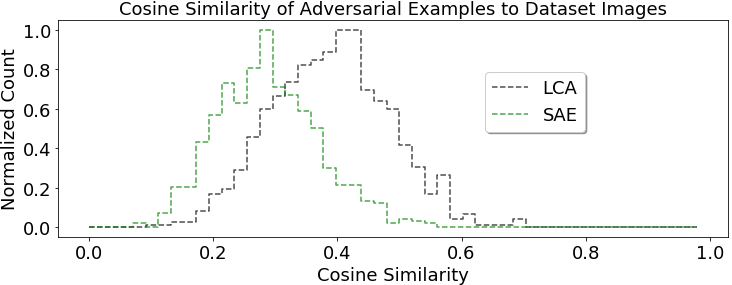
\includegraphics[width=0.9\textwidth]{figures/cosyne_similarity.png}
    \caption{\textbf{Adversarial attacks using gradients from the LCA have a larger cosine similarity to dataset images than attacks for the SAE.} Following \parencite{kos2018adversarial, kurakin2016adversarial}, we attacked each model using a target image that had an alternate class label. The histograms are computed over 800 image examples.}
    \label{fig:ch4_cosine_similarity}
\end{figure}

In addition to being data-aligned, we found that the sigmoid nonlinearity in particular was susceptible to unbounded adversarial attacks. To demonstrate this, we again followed the iterative fast sign gradient method from \parencite{kurakin2016adversarial} but applied to the generative adversarial models as is done in \parencite{kos2018adversarial}. We additionally removed the clipping step and allowed the perturbation vector to grow without bound. Figure \ref{fig:ch4_lca_sae_unbounded_attack} shows that the LCA is protected against this unbounded attack and the vector ultimately settles on some length. However, the perturbation vector for the SAE model continues to grow, which we hypothesize is a consequence of the sigmoid nonlinearity.

\begin{figure}
    \centering
    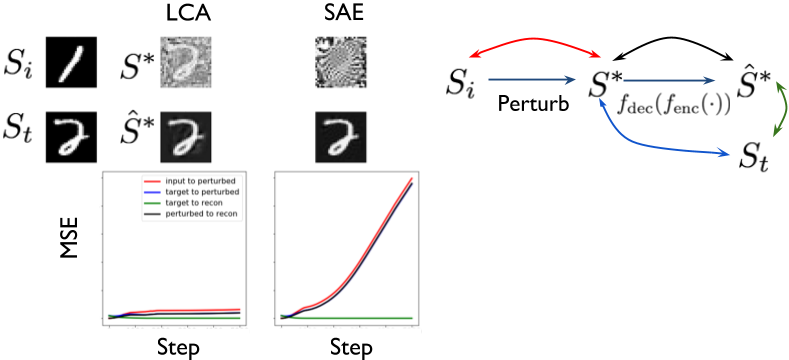
\includegraphics[width=\textwidth]{figures/lca_sae_unbounded_attack.png}
    \caption{\textbf{The LCA is protected against unbounded adversarial attacks.} We attack a single layer sparse autoencoder and the LCA network with an unbounded Kurakin attack \parencite{kurakin2016adversarial}. The attack is able to find a perturbation direction for the SAE model that can grow without bound while producing an approximately equivalent reconstruction. However, with the LCA model the attack converges and the perturbation vector is unable to continue to grow.}
    \label{fig:ch4_lca_sae_unbounded_attack}
\end{figure}


%TODO: 
%\subsubsection{LCA is robust against transferred adversarial attacks}
%To understand how adversarial attacks transfer between these models, we produced adversarial images for each one and test how adversaries generated for one model affect another.
%The data-aligned perturbations can explain why adversarial images for LCA transfer to SAE and VAE but not the other way around \ref{fig:figure}.


% TODO:
%\subsubsection{Pixel classification attack}
%The standard attack method for classification networks is to perturb input pixels to result in misclassification. One proposed defense against this type of attack is to preprocess the image pixels with a denoising autoencoder that would produce reconstructions void of the adversarial pixel perturbations. However, it has been shown that if one backpropagates the adversarial loss through the autoencoder network, then it is still possible to adversarially attack the network. Here we show that the LCA model outperforms the VAE and SAE networks as a preprocessing ``firewall'' against the adversarial attacks.

\subsubsection{Replacing the first layer of an MLP with an LCA layer boosts robustness}
In chapter 3 we discussed potential benefits of using LCA as an unsupervised training method for semi-supervised classification tasks. %TODO: Fix chapter refs
Here, we show that the same network setup as we described in section \ref{sec:ch3_weak_supervised_learning} has additional robustness to adversarial attacks.
Although we did not include feedback during inference in our adversarial experiments, we do identify this as a promising direction for future work.
In this experiment we first trained a two-layer fully-connected ReLU (MLP) model on the MNIST dataset as our control.
Our comparison model is the LCA trained without supervision and a single-layer perceptron (SLP) classifier trained on LCA activations.
Both models were trained to have comparable validation accuracy.
Figure \ref{fig:ch4_adversarial_mlp_vs_lca} gives the original input to perturbed image MSE for three attack types: most-likely adversarial targeted, least-likely adversarial targeted, and untargeted.
The first attack type takes the second highest candidate class (in terms of the softmax confidence output) and adversarially perturbs the input to that class.
The second type takes the lowest candidate class and perturbs to it.
The third attack minimizes the negative of the original cross-entropy training loss.
The figure also shows reconstructions for a ``7'' digit adversarially perturbed to a ``6''.
It is plain to see that for equal confidence the LCA+SLP model requires more semantically significant perturbations in that the perturbed image looks much more like a ``6''.
%TODO: This ties in with the sabor / hinton dark-net result. the capsule net also has pop nl and therefore might exhibit exo-bent contours.
%TODO: Also should elaborate more on this result - mention the generative model argument again?
This result was consistent for many of the attack images that we sampled.

\begin{figure}
    \centering
    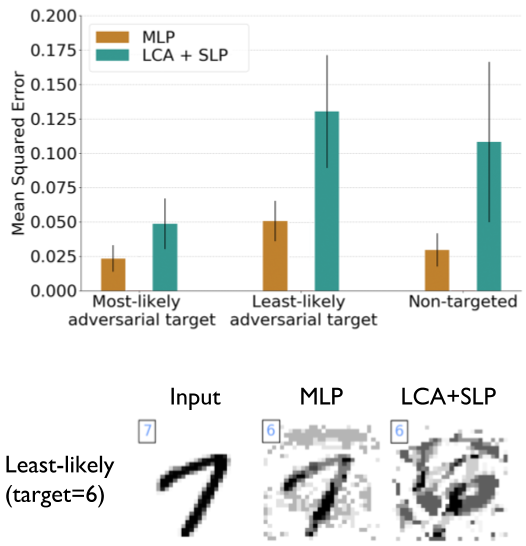
\includegraphics[width=0.5\textwidth]{figures/adversarial_mlp_lca_slp.png}
    \caption{\textbf{LCA protects against traditional adversarial attacks.} Here we perform three types of attacks based on the iterative fast sign gradient method \parencite{kurakin2016adversarial, kos2018adversarial}. For all three types of attacks the LCA + SLP network outperforms the equal-sized MLP network. Both were trained to comparable validation accuracy. The lower images are example adversarial attacks with equal classification confidence. The blue digit in the top left indicates the original label for the left-most image and the adversarial target for the right two images.}
    \label{fig:ch4_adversarial_mlp_vs_lca}
\end{figure}


\subsubsection{Generative adversarial attacks}
Results from \parencite{kos2018adversarial, gondim2018adversarial, goodfellow2014explaining} show that adversarial stimulus can be constructed for generative models. This is especially compelling because generative models are explicitly trained to preserve information about the input and produce a veridical reconstruction, whereas classification networks are typically trained to throw away large amounts of information and only preserve that which is relevant for the given task. We show that the LCA model is robust against generative adversarial attacks when compared to the deep ReLU AE, SAE \parencite{ng2011sparse} and VAE \parencite{kingma2013auto} networks.

For the first generative attack, an input image, $s$, was minimally perturbed before being passed through the autoencoder to produce a reconstruction of an entirely different target image, $s_{t}$. We reproduced the Carlini style attack \parencite{carlini2017towards, kos2018adversarial} using the following equation:

\begin{equation}\label{eq:ch4_kos_carlini_attack}
    \mathcal{L} = \tfrac{1}{2} \|s_{t} - \hat{s}^{*}\|_{2}^{2} + \tfrac{\alpha}{2}\|s - s^{*}\|_{2}^{2}.
\end{equation}

The LCA shows robustness against this attack in that the adversarial input has a strong resemblance to the target output category, or the input and output look like a superposition of the two classes. However, for the deep rectified autoencoder, it was possible to produce an attack which had an input that can be identified as one class and an output that is identified as an alternate class. We demonstrate this result in figure \ref{fig:ch4_carlini_deep_relu_lca}.

\begin{figure}[h]
    \centering
    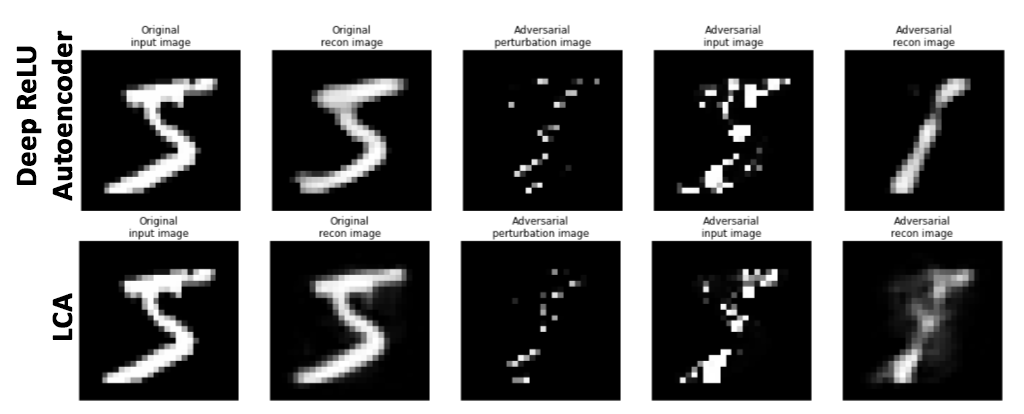
\includegraphics[width=\textwidth]{figures/adv_carlini_deep_relu_lca.png}
    \caption{\textbf{Generative adversarial attacks succeed on deep rectified networks but fail on the LCA.} The deep rectified network can be attacked such that the input resembles one digit class and the output resembles another. Single-layer autoencoders (not shown) and the LCA are protected against this attack. The attack follows the methods outlined in \parencite{kos2018adversarial} and equation \eqref{eq:ch4_kos_carlini_attack}.}
    \label{fig:ch4_carlini_deep_relu_lca}
\end{figure}

For the second generative attack, the perturbation was done by minimizing a loss that resembles equation \eqref{eq:ch4_kos_carlini_attack}, but modifies the trade-off parameter to be a balanced weighting between the perturbation magnitude and the distance between the reconstruction and the target:

\begin{equation}\label{eq:ch4_carlini_targeted_recon}
    \mathcal{L} = \tfrac{\alpha}{2} \|s_{t} - \hat{s}^{*}\|^{2} + \tfrac{1-\alpha}{2}\|s - s^{*}\|^{2}.
\end{equation}

\noindent where $s^{*}=s+e$ is the perturbed image. This modification allows us to sweep the $\alpha$ parameter between the two loss terms. We show in figure \ref{fig:ch4_kos_generative_attack} that the LCA outperforms the comparison models for all parameters tested.

%TODO: Verify this plot - number of images? standard deviation?
\begin{figure}[h]
    \begin{center}
    \centerline{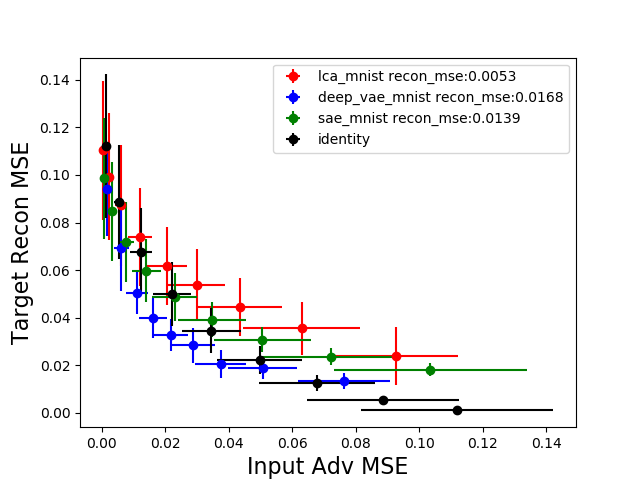
\includegraphics[width=\columnwidth]{figures/recon_mult_tradeoff.png}}
    \end{center}
    \caption{\textbf{LCA protects against MNIST generative adversarial attacks.} The Carlini-style generative attack introduced in \parencite{kos2018adversarial} has a trade-off parameter for importance between the target image to reconstruction MSE and the input image to perturbed image MSE. When we sweep this parameter using the loss defined in equation \eqref{eq:ch4_carlini_targeted_recon}, we find that the LCA consistently outperforms comparison models. The numbers in the labels represent the average reconstruction MSE for each model. Error bars indicate standard deviation for 100 images.}
    \label{fig:ch4_kos_generative_attack}
\end{figure}


\subsubsection{Comparing to the LISTA network}
The lateral connectivity in the LCA network is implemented via a recurrent computation. These dynamics facilitate a form of explaining away, where neurons that have a high degree of correspondence with the input stimulus suppress other neurons in the network. This results in the network ignoring input pixels that are not aligned with primary data directions. To better understand the role of the recurrent computation, we trained a network that acts as an unrolled version of LCA, where the lateral connectivity and feedforward weight matrices are learned. The LISTA model is a recurrent network with many fewer inference steps that can produce codes that have a small Euclidean distance to the outputs of sparse coding \parencite{gregor2010learning}. We trained three LISTA models with 5, 20, and 50 layers. All three models were trained to produce codes that had approximately the same $l_{2}$ distance from the codes produced by 50 steps of LCA inference. We show in figure \ref{fig:ch4_adversarial_lista_vs_lca} that the LISTA network does not perform as well as LCA at defending against adversarial attacks and that the deeper LISTA networks perform no better. The attacks follow methods in (\cite{carlini2017towards}, ``Carlini'' targeted attack) and (\cite{kurakin2016adversarial}, ``Kurakin'' untargeted attack). For the Carlini attack we ran 10,000 steps with a step size of 0.001 and report the resulting MSE. The average adversarial confidences for the Carlini attack were 55\%, 55\%, 56\%, and 48\% for LISTA 5, 20, 50, and LCA, respectively. For the Kurakin attack we run the attack until it reaches an average adversarial confidence of $\sim 95$\%. 

\begin{figure}[h]
    \centering
    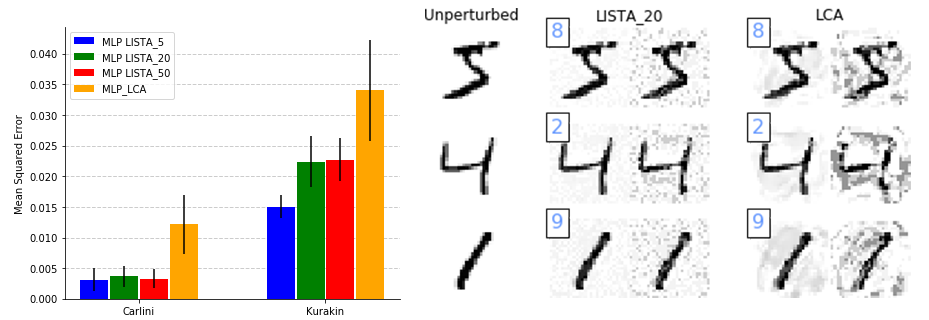
\includegraphics[width=\textwidth]{figures/adversarial_lista_vs_lca.png}
    \caption{\textbf{LCA protects better than LISTA against latent classification attacks.} We generated adversarial examples from equal-sized MLPs trained from the latent codes of each model. MSEs were calculated between the original image and the perturbed image. Error bars indicate standard deviation for 100 example inputs. The images on the right show the resulting adversarial attacks. The left most column are the original unperturbed images. The next column has adversarially perturbed inputs the 20 layer LISTA model using the Carlini method. Next are perturbed inputs using the Kurakin method. The fourth column are adversarially perturbed images using the Carlini method on the LCA model. The final column are adversarially perturbed images using the Kurakin method on the LCA model. The blue digit in the top left of the Carlini attack images is the target digit class for each adversarial attack.}
    \label{fig:ch4_adversarial_lista_vs_lca}
\end{figure}


%TODO:
%\subsubsection{Attacks with the CIFAR dataset}
%The LCA objective is derived from a model of natural images, so we believe the network will exhibit stronger aversion to adversarial perturbations.



%TODO:
%\section{Explaining extra-classical receptive field effects}
% explain Golden stuff; note zhu results
% compare zhu reproduced results to ica


%TODO:
%\section{Applications to physiological neuroscience}
%Use this method to probe neuron contours.


\subsection{Discussion}
Although the softmax nonlinearity used in most classification models is a population nonlinearity, it has little effect on the computation performed by the neural network as it can be, and is, without loss of generality, incorporated into the loss function. We hypothesize that the deep network does not produce consistently exo-origin bent contours in class-relevant data directions, which will result in more adversarial susceptibility.
% TODO:
% talk about generative robustness, the LCA performs as well as a deep AE but does not have additional sucept to adv atk
%Single-layer autoencoders (not shown) and the LCA are protected against this attack.

Additional control models need to be explored, including alternative population nonlinearities such as those present in Boltzmann machines \parencite{salakhutdinov2009deep}, divisive normalization \parencite{balle2016end}, and local response normalization \parencite{krizhevsky2012imagenet}. Each of these nonlinearities has had significance in the deep learning and neuroscience communities. The iso-response analysis provides a methodology for contrasting them and will give us valuable insight into how each of them may respond to adversarial attacks. We also wish to scale up the models to include larger datasets of more naturalistic images. 

The hierarchical extension to the sparse coding model proposed in \parencite{chen2018sparse} has been shown to perform a better job of mapping input data onto a smooth manifold. We hypothesize that this will further increase the semantic relevance of attacks and model robustness against adversarial perturbations. We identify the model defined in \parencite{chen2018sparse} as a candidate for exploring how the adversarial and iso-response properties change as we increase the network depth.

This methodology has a high potential for impact in the deep learning community. We advocate for biologically motivated computations that go beyond the simple pointwise nonlinear model. We have shown that these types of networks learn a more robust representation of data without tedious and biased human labeling. We also provide strong theoretical support for our hypotheses and an analysis method that allows us to fully characterize how the more complicated neurons will respond to input perturbations.

\section{Conclusion}
In this chapter we expanded on a recently proposed method for understanding neurons by measuring their response geometry. While earlier work only demonstrated neuron response contours on toy datasets with very low dimensional stimulus, we outlined a scalable method for computing neuron iso-response contours on image patches and MNIST digits. Additionally, we performed a population-level analysis to show that the LCA has exo-origin bent contours in almost all orthogonal directions. We provide evidence supporting hypotheses from the literature that exo-origin curvature is indicative of a higher degree of selectivity and efficiency. Finally, we propose that the response contours can be used to predict iso-response directions. We provide a mathematical justification as well as experimental support for this hypothesis.